\documentclass[varwidth=true,crop=false]{standalone}
\usepackage[chatter]{rotating}
\usepackage{amssymb,amsmath}
\usepackage{pgfplots}

\usepackage{geometry}
\geometry{
paperwidth=12in,
paperheight=12in,
margin=0.25in
}

\newcommand{\pisub}[1]{\pi_{\mathrm{#1}}}
\newcommand{\pilow}{\pisub{low}}
\newcommand{\pihigh}{\pisub{high}}
\newcommand{\piI}{\langle \pisub{I} \rangle}
\newcommand{\piS}{\langle \pisub{S} \rangle}
\newcommand{\ledger}{\bar\pi_{ib}}

\newcommand{\meanvar}[1]{\langle #1 \rangle}
\newcommand{\meansl}{\meanvar{s}}
\newcommand{\meanpi}{\meanvar{\pi}}
\newcommand{\meansoc}{\meanvar{\pi_\mathrm{S}}}
\newcommand{\meanasoc}{\meanvar{\pi_\mathrm{A}}}
\newcommand{\meanT}{\meanvar{T}}

\newcommand{\bandit}{\text{Bandit}_b(0, 1)}

\begin{document}
% \begin{tikzpicture}
      % \draw[->,thick] (-.1,0)--(1.15,0) node[above]
      %   {\huge Selection-set size};
      %   % {Number of behaviors $B$};
      % \draw[->,thick] (0,.1)--(0,-1.15) node[below]
      %   {\huge Low payoff\\(payoff ambiguity proxy)};
      %   % {Low payoff frequency $\pilow$};
	  % \end{tikzpicture}~\\[2em]

    \begin{minipage}{3.75in}
      \centering
      {\hspace{5.25em}\huge Selection-set size$ = 2$}
    \end{minipage}%
    \begin{minipage}{3.75in}
      \centering
      {\hspace{3.0em}\huge Selection-set size$ = 4$}
    \end{minipage}%
    \begin{minipage}{3.75in}
      \centering
      {\hspace{3.0em}\huge Selection-set size$ = 10$}
    \end{minipage}~\\

    \begin{minipage}{3.75in}
    \begin{rotate}{90}
      {\parbox{3.0in}{
          \centering
          \vspace{-1.0em}\hspace{-2.5em} {\huge Low payoff $ = 0.1$} \\[1em]
          {\huge SL fixation frequency}
      }}
    \end{rotate}%
    \hspace{2em}
      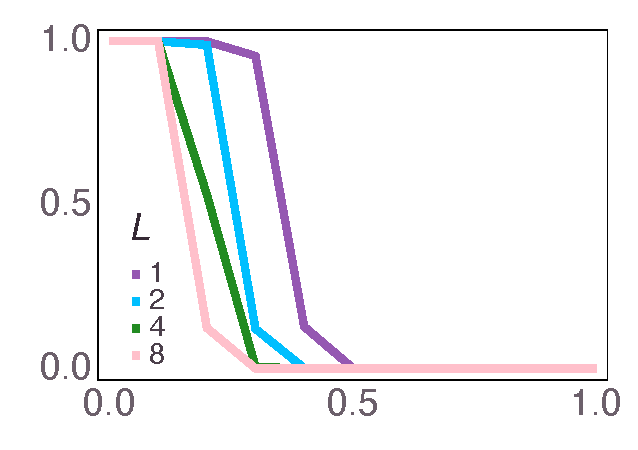
\includegraphics[width=\textwidth]{Figures/mean_social_learner_over_u_lowpayoff=0.1_nbehaviors=2.pdf}
    \end{minipage}\noindent\hspace{1.25em}
	\begin{minipage}{3.75in}%
      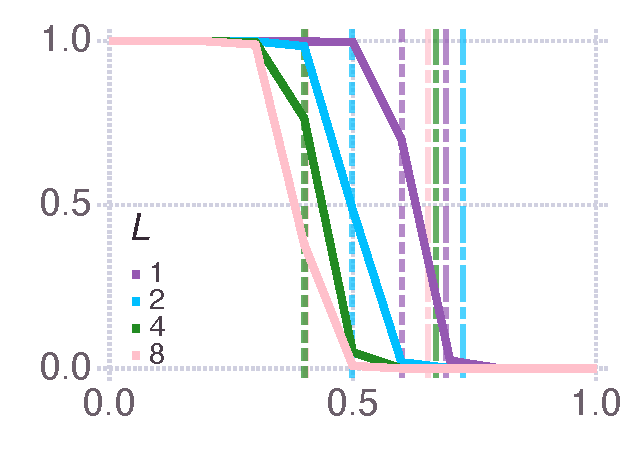
\includegraphics[width=\textwidth]{Figures/mean_social_learner_over_u_lowpayoff=0.1_nbehaviors=4.pdf}
    \end{minipage}\noindent
	\begin{minipage}{3.75in}%
      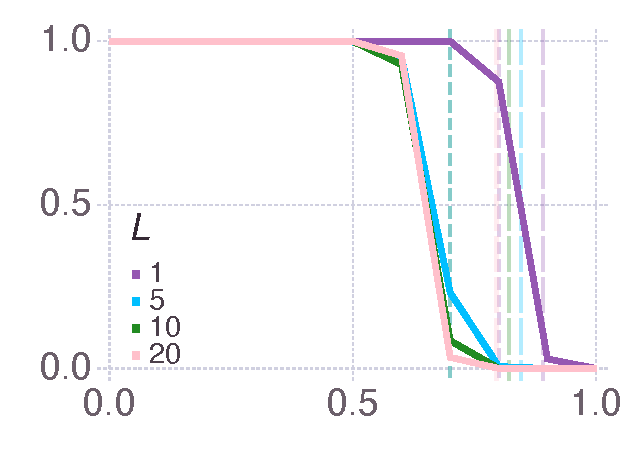
\includegraphics[width=\textwidth]{Figures/mean_social_learner_over_u_lowpayoff=0.1_nbehaviors=10.pdf}
    \end{minipage}~\\[2.5em]

    \begin{minipage}{3.75in}
    \begin{rotate}{90}
      {\parbox{3.0in}{
          \centering
          \vspace{-1.0em}\hspace{-2.5em} {\huge Low payoff $ = 0.45$} \\[1em]
          {\huge SL fixation frequency}
      }}
    \end{rotate}%
    \hspace{2em}
      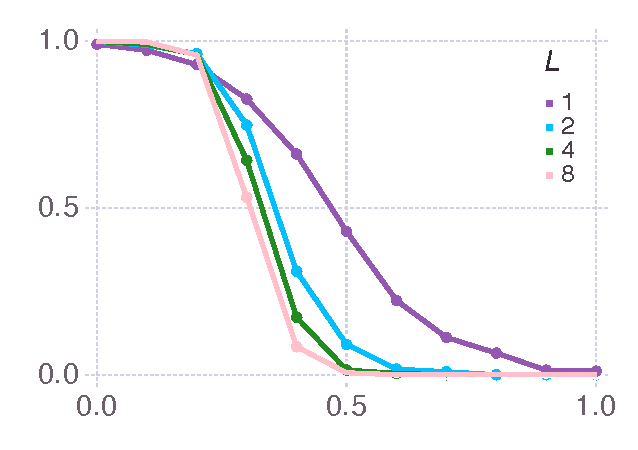
\includegraphics[width=\textwidth]{Figures/mean_social_learner_over_u_lowpayoff=0.45_nbehaviors=2.pdf}
	\end{minipage}\noindent\hspace{1.25em}
	\begin{minipage}{3.75in}%
      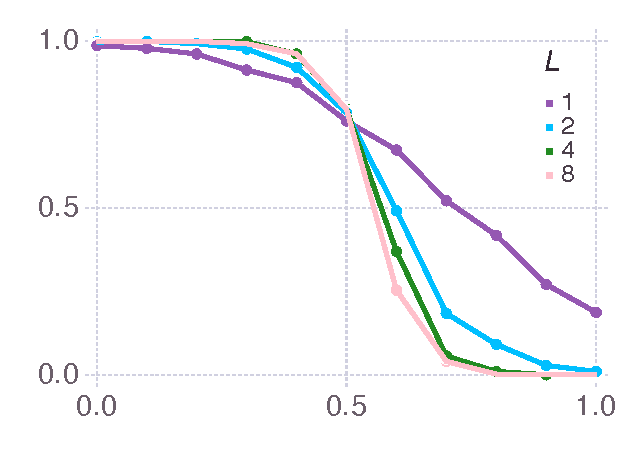
\includegraphics[width=\textwidth]{Figures/mean_social_learner_over_u_lowpayoff=0.45_nbehaviors=4.pdf}
    \end{minipage}\noindent
	\begin{minipage}{3.75in}%
      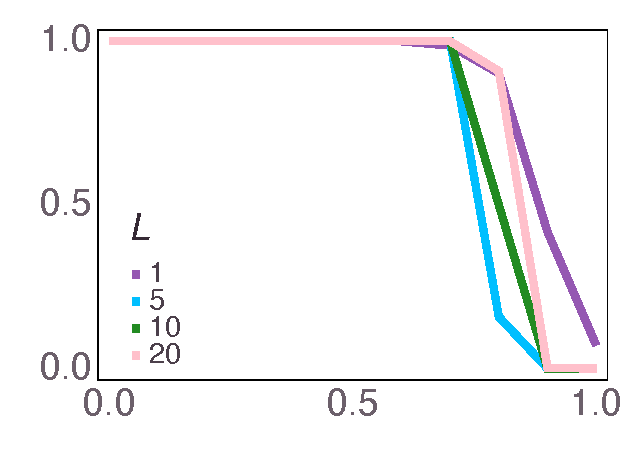
\includegraphics[width=\textwidth]{Figures/mean_social_learner_over_u_lowpayoff=0.45_nbehaviors=10.pdf}
    \end{minipage}~\\[2.5em]

    \begin{minipage}{3.75in}
    \begin{rotate}{90}
      {\parbox{3.0in}{
          \centering
          \vspace{-1.0em}\hspace{-2.5em}{\huge Low payoff $= 0.8$} \\[1em]
          {\huge SL fixation frequency}
          % {\begin{rotate}{-90}{\huge $\meansl$}\hspace{3em}\end{rotate}}
      }}
    \end{rotate}%
    \hspace{2em}
      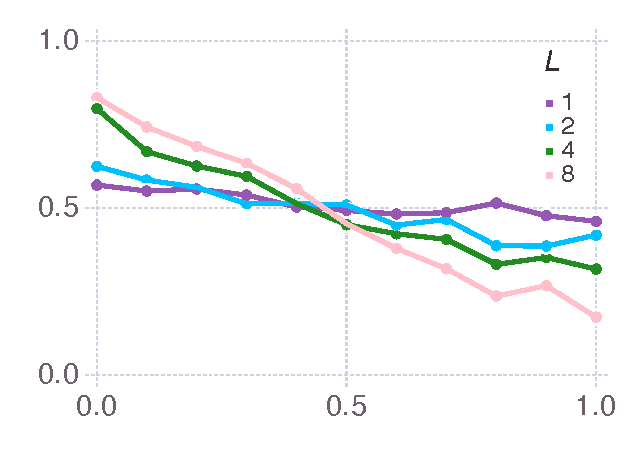
\includegraphics[width=\textwidth]{Figures/mean_social_learner_over_u_lowpayoff=0.8_nbehaviors=2.pdf}
        \\[-2.75em]
        \begin{center}
          {\hspace{3.25em} \huge Environmental variability}
      \end{center}
	  \end{minipage}\noindent\hspace{1.25em}
		\begin{minipage}{3.75in}%
		  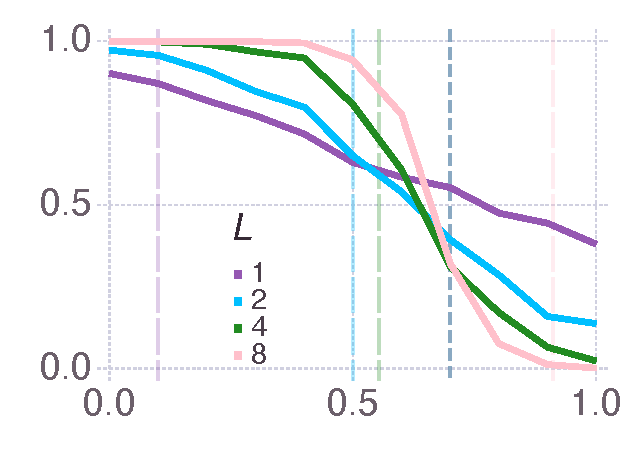
\includegraphics[width=\textwidth]{Figures/mean_social_learner_over_u_lowpayoff=0.8_nbehaviors=4.pdf}
		  \\[-2.75em]
	  \begin{center}
          {\hspace{3.25em} \huge Environmental variability}
      \end{center}
    \end{minipage}
	\begin{minipage}{3.75in}%
		  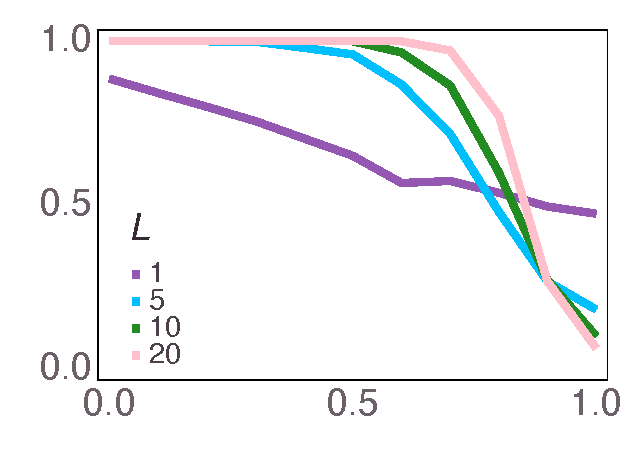
\includegraphics[width=\textwidth]{Figures/mean_social_learner_over_u_lowpayoff=0.8_nbehaviors=10.pdf}
		  \\[-2.75em]
	  \begin{center}
          {\hspace{3.25em} \huge Environmental variability}
      \end{center}
    \end{minipage} 
    % \\[2.5em]
    % \begin{center}
    %   
\includegraphics[width=1.85in]{Figures/legendElements/ldashdot.pdf}
    %   {\Huge$\meanasoc = \meansoc$} \quad \quad
    %   
\includegraphics[width=1.85in]{Figures/legendElements/dot.pdf}
    %   {\Huge$\underset{u}{\arg\max}~\langle G(u) \rangle$}
    % \end{center}
\end{document}
